% -----------------------------------------------
% Template for ISMIR Papers
% 2015 version, based on previous ISMIR templates
% -----------------------------------------------

\documentclass{article}
\usepackage{ismir,amsmath,cite}
\usepackage{graphicx}
\usepackage{color}
\usepackage{mathrsfs}
\usepackage[english]{babel}
\usepackage{caption}
\usepackage{subfig, color}
\usepackage{microtype}
\usepackage{IEEEtrantools}
\sloppy

\usepackage{xspace}
\newcommand*{\eg}{e.g.\@\xspace}
\newcommand*{\ie}{i.e.\@\xspace}
\newcommand*{\etal}{\emph{et al.}\@\xspace}

% Title.
% ------
\title{Learning pitch invariants for instrument recognition}


% Single address
% To use with only one author or several with the same address
% ---------------
\oneauthor
{Names should be omitted for double-blind reviewing}
{Affiliations should be omitted for double-blind reviewing}
%\oneauthor
%{Vincent Lostanlen, Carmine Emanuele Cella, and St\'{e}phane Mallat}
%{\'{E}cole normale sup\'{e}rieure}

% Two addresses
% --------------
%\twoauthors
%  {First author} {School \\ Department}
%  {Second author} {Company \\ Address}

% Three addresses
% --------------
%\threeauthors
 %{First author} {Affiliation1 \\ {\tt author1@ismir.edu}}
 %{Second author} {\bf Retain these fake authors in\\\bf submission to preserve the formatting}
 %{Third author} {Affiliation3 \\ {\tt author3@ismir.edu}}

% Four addresses
% --------------
%\fourauthors
%  {First author} {Affiliation1 \\ {\tt author1@ismir.edu}}
%  {Second author}{Affiliation2 \\ {\tt author2@ismir.edu}}
%  {Third author} {Affiliation3 \\ {\tt author3@ismir.edu}}
%  {Fourth author} {Affiliation4 \\ {\tt author4@ismir.edu}}

\begin{document}
%
\maketitle
%
\begin{abstract}
Musical performance combines a wide range of pitches, nuances,
and expressive techniques.
Audio-based classification of musical instruments thus requires to
build signal representations that are invariant to such transformations.
Focusing on pitch invariance, this article investigates the construction
of multi-stage architectures for instrument recognition.
% Missing sentence
We show that Mel-frequency cepstral coefficients (MFCC) lack
invariance with respect to realistic pitch shifts.
In turn, a convolutional neural network (ConvNet) in the time-frequency
domain is able to disentangle pitch from timbral information in a subtler way.
We extend our method to the recognition of multiple instruments playing simultaneously.
\end{abstract}

\section{Introduction}\label{sec:introduction}
Among the cognitive attributes of musical tones, pitch is distinguished
by a combination of three properties.
First, it is relative: ordering pitches from low to high gives rise to
intervals and melodic patterns.
Secondly, it is intensive: multiple pitches heard simultaneously produce
a chord, not a single unified tone -- contrary to loudness, which adds
up with the number of sources.
Thirdly, it does not depend on instrumentation: this makes possible
the transcription of polyphonic music under a single symbolic system \cite{Krumhansl2001}.

Tuning auditory filters to a perceptual scale of pitches provides a
time-frequency representation of music signals that satisfies the first two of these properties.
It is thus a starting point for a wide range of MIR applications,
which can be separated in two categories: pitch-\emph{relative}
(\eg chord estimation \cite{Humphrey2012})
and pitch-\emph{invariant} (\eg instrument recognition \cite{Eronen2000}).
Both aim at disentangling pitch from timbral content as independent
factors of variability, a goal that is made possible by the third aforementioned property.
This is pursued by extracting mid-level features on top of the spectrogram,
be them engineered or learned from training data.
Both approaches have their limitations: a "bag-of-features" lacks flexibility
to represent fine-grain class boundaries, whereas a purely learned pipeline
often leads to uninterpretable overfitting, especially in MIR where the quantity
of thoroughly annotated data is relatively small.

In this article, we strive to integrate domain-specific knowledge about musical
pitch into a deep learning framework, hence bridging the gap between feature
engineering and feature learning.

%Deep convolutional networks have proven to disentangle factors of variability
%among natural images, such as pose, color, and lighting conditions.

Section 2 reviews the related work on feature learning for signal-based music
classification.
Section 3 demonstrates that pitch is the major factor of variability among musical
notes of a given instrument, if described by their mel-frequency cepstra.
Section 4 describes a typical deep learning architecture for spectrogram-based
classification, consisting of two convolutional layers and one densely connected layer.
Section 5 improves the previous architecture by splitting spectrograms into
octave-wide frequency bands, training specific convolutional layers over each band
in parallel, and gathering feature maps at a later stage.
Sections 6 discusses the effectiveness of the presented systems on a challenging
dataset for music instrument recognition.

\section{Related work}
Spurred by the growth of annotated datasets and the democratization of
high-performance computing, feature learning has enjoyed a renewed interest
in recent years within the MIR community.

For music instrument recognition: \cite{McFee2015-muda}, \cite{Li2015}.

Some other applications include onset detection \cite{Schluter2014},
transcription \cite{Sigtia2015}, genre classification \cite{Choi2015},
chord recognition \cite{Humphrey2012}, boundary detection \cite{Ullrich2014}, and
recommendation \cite{vandenOord2013}.

The most widely studied deep learning system for music information retrieval consists of two convolutional layers and two densely connected layers, with minor variations \cite{Humphrey2012, Kereliuk2015, Li2015, McFee2015-muda, Schluter2014, Ullrich2014}.
% The problem is made difficult by the fact that factors of variability are entangled.
% Deep convolutional networks have proven to disentangle factors of variability in computer
% vision, such as pose, color, and lighting conditions.

% the challenge is thus two-fold
% 1. gaining abstraction by integrating time-frequency patterns over longer time scales
% 2. building invariants to melody while remaining highly discriminative to the instrument

% On music instrument classification
% Ref to Joder et al
% Ref to Fuhrmann
% On feature learning
% Ref to Dieleman and Benjamin ICASSP 2014
% Ref to Humphrey, Bello, LeCun 2012
% Ref to Salamon and Bello
% Ref to Li, Qian, and Wang arXiv 2015
% Ref to Simpson

\section{How invariant is the Mel-frequency cepstrum ?}
The mel scale is a quasi-logarithmic function of acoustic frequency designed such that
perceptually similar pitch intervals appear equal in width over the full hearing range.
This section shows that engineering transposition-invariant features from the mel
scale does not suffice to build pitch invariants for complex sounds, thus motivating
further inquiry.

The time-frequency domain produced by a constant-Q filter bank tuned to the mel
scale is covariant with respect to pitch transposition of pure tones.
As a result, a chromatic scale played at constant speed would draw parallel,
diagonal lines, each of them corresponding to a different partial wave.

However, the physics of musical instruments constrain these partial waves to bear
a negligible energy if their frequencies are beyond the range of acoustic resonance.

This implies that realistic pitch changes cannot be modeled by translating a rigid
spectral template along the log-frequency axis.
The same property is verified for a wide class of instruments, especially brass and
woodwinds.  

\begin{figure}[t]
    \begin{center}
        \setlength{\unitlength}{1cm}
        \begin{picture}(8.5,3.2)
        \put(0.1,0){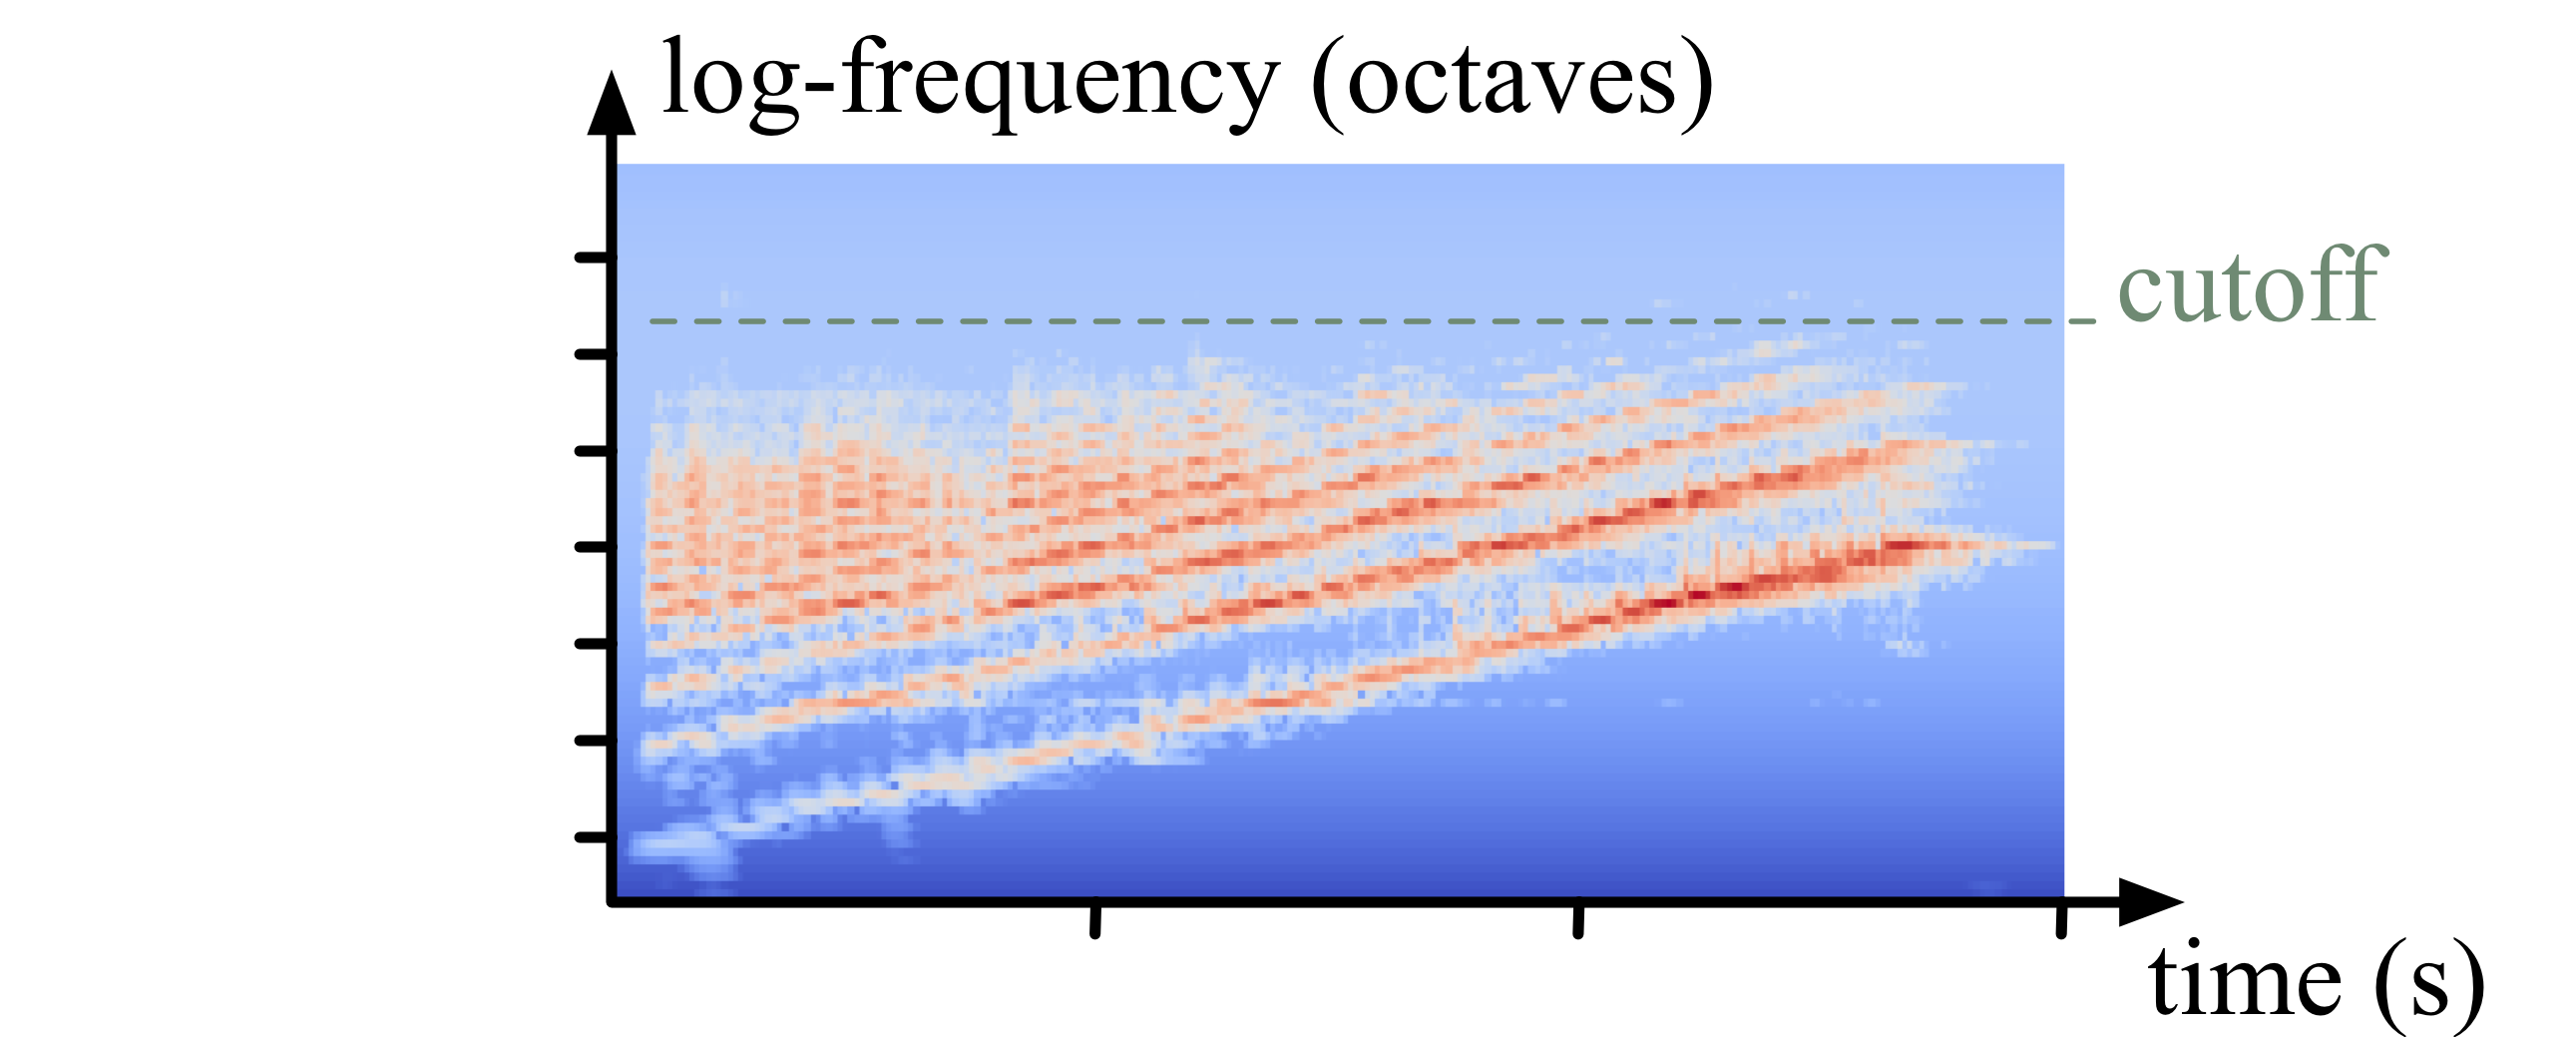
\includegraphics[width=8cm]{figs/chromatic_scale.png}}
        \end{picture}
    \end{center}
    \protect\caption{
    Constant-Q spectrogram of a chromatic scale played by a tuba.
    Although the harmonic partials shift progressively, the spectral envelope remains unchanged,
    as revealed by the presence of a fixed cutoff frequency.
    See text for details.
\label{fig:mfcc-variances}
}
\end{figure}

Following a well-established rule, the MFCC were extracted by computing
the discrete cosine transform (DCT) from a mel-frequency spectrum of 40 bands
with logarithmic compression of loudness, and keeping its 13 lowest "quefrencies".

We found that the MFCC cluster corresponding to each instrument is shrinked if
decomposed into a mixture of same-pitch clusters, sometimes by an order of
magnitude.
In other words, most of the variance in an instrument cluster of mel-frequency
cepstra is due to pitch transposition.
This experiment shows that the mel-frequency cepstrum lacks invariance to realistic
pitch shifts, and that there remains a lot to be gained by feature learning in this area.

\begin{figure}[t]
    \begin{center}
        \setlength{\unitlength}{1cm}
        \begin{picture}(8.5,8.7)
        \put(0.1,0){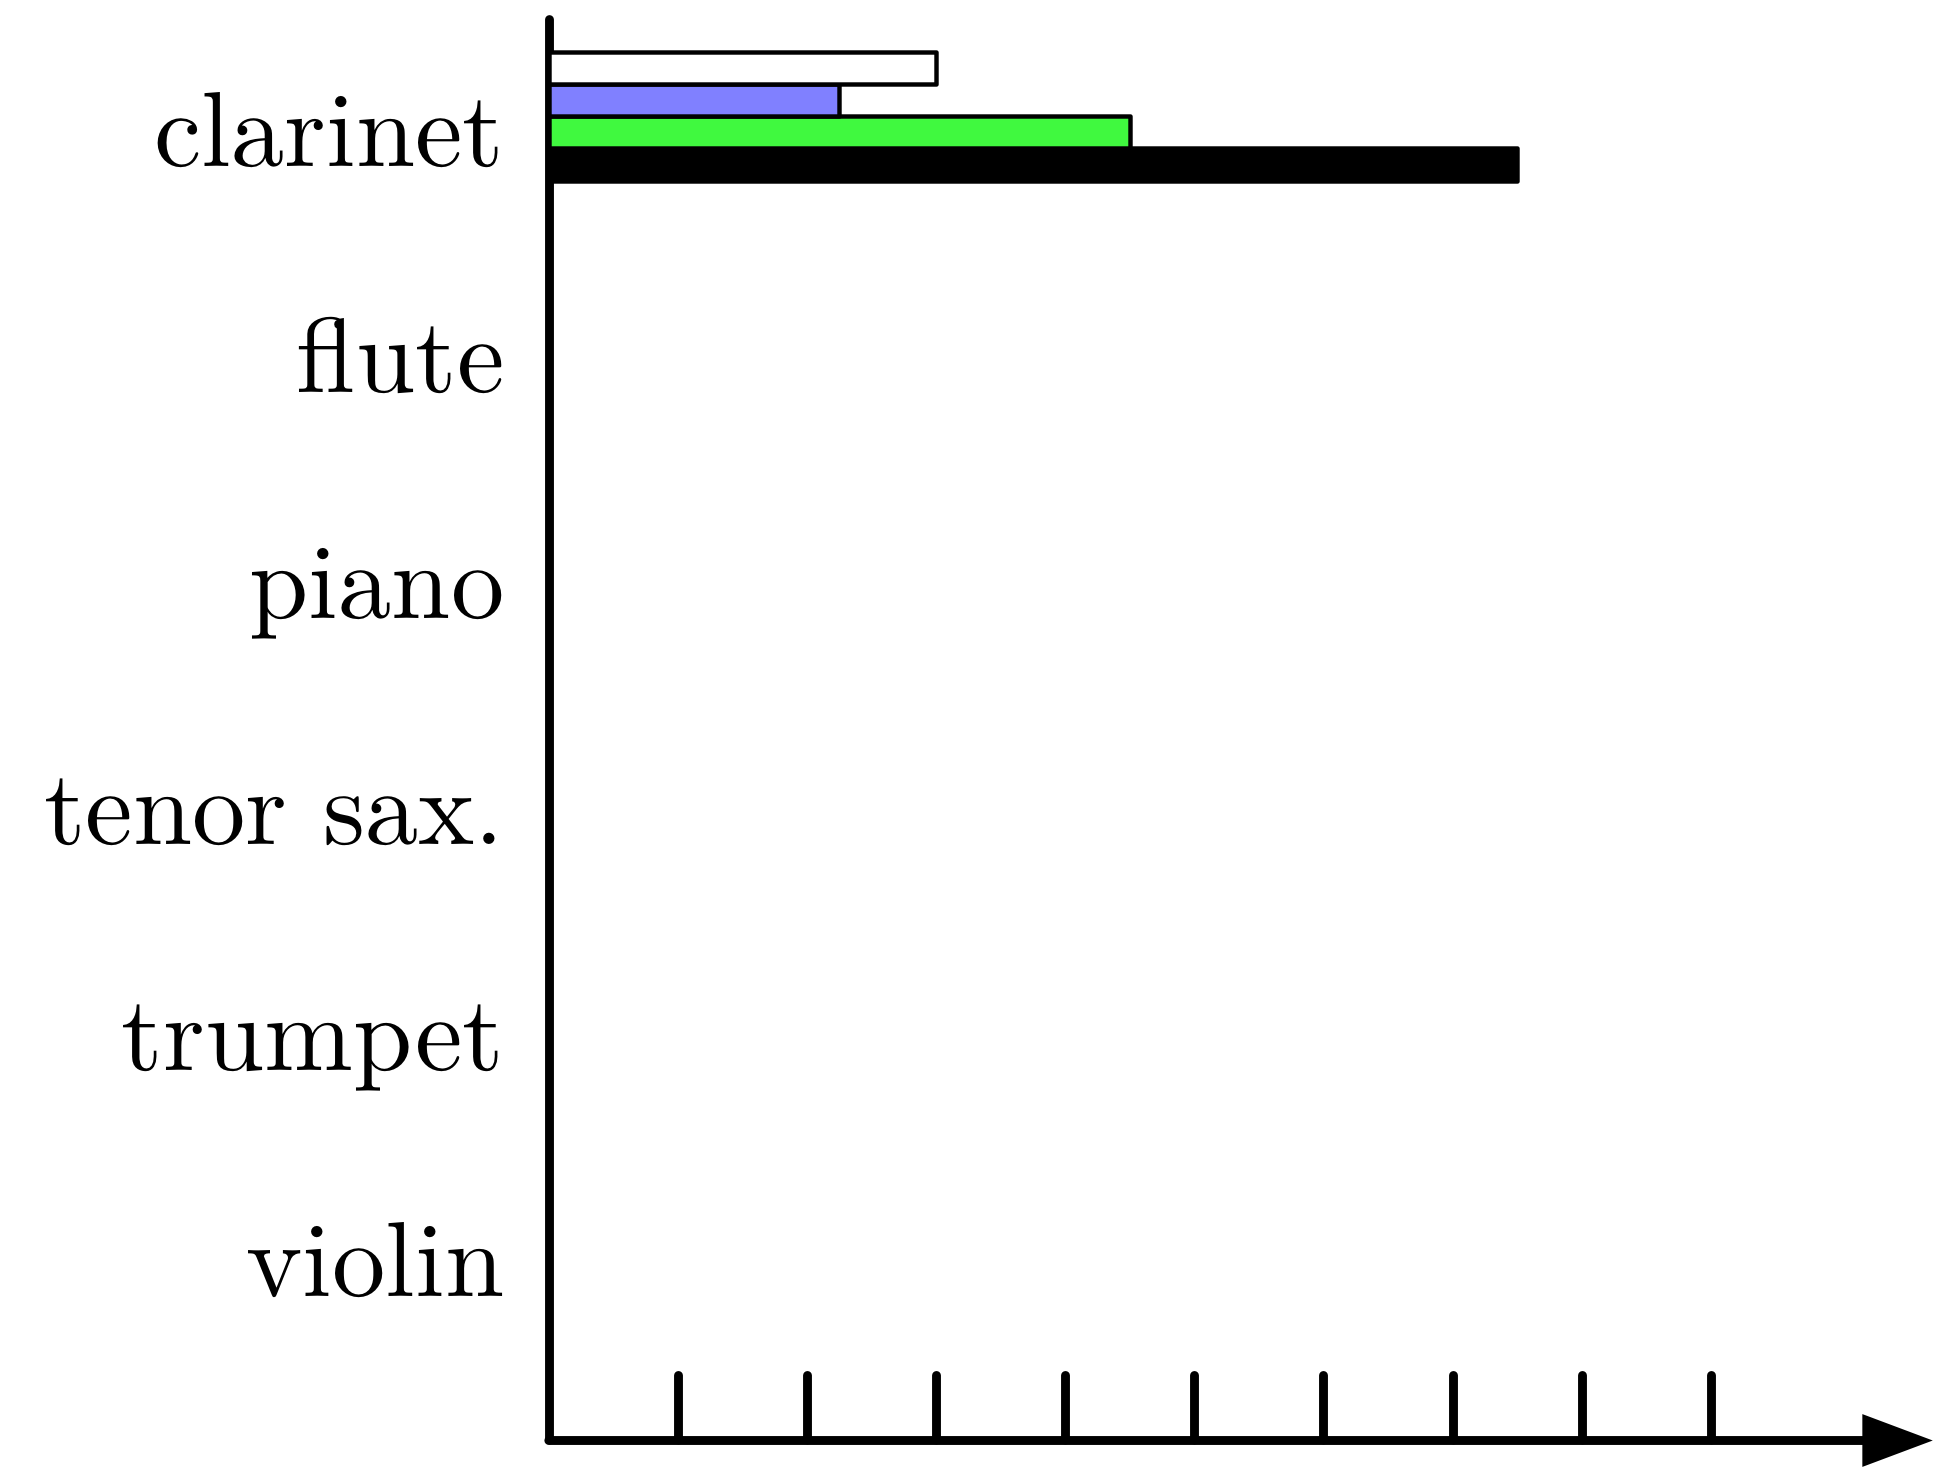
\includegraphics[width=8cm]{figs/mfcc_variances.png}}
        \end{picture}
    \end{center}
    \protect\caption{
Distributions of squared Euclidean distances among various MFCC clusters in the RWC dataset. Whisker ends denote lower and upper deciles. See text for details.
\label{fig:mfcc-variances}
}
\end{figure}
 
\section{Deep convolutional networks}
A deep learning system for classification is built by stacking multiple layers of weakly nonlinear transformations, whose parameters are jointly optimized such that the top-level layer fits a training set of labeled examples.
This section introduces a typical deep learning architecture for audio classification and describes the functioning of each layer.

\begin{figure*}[t]
    \begin{center}
        \setlength{\unitlength}{1cm}
        \begin{picture}(17,5)
        \put(0,0){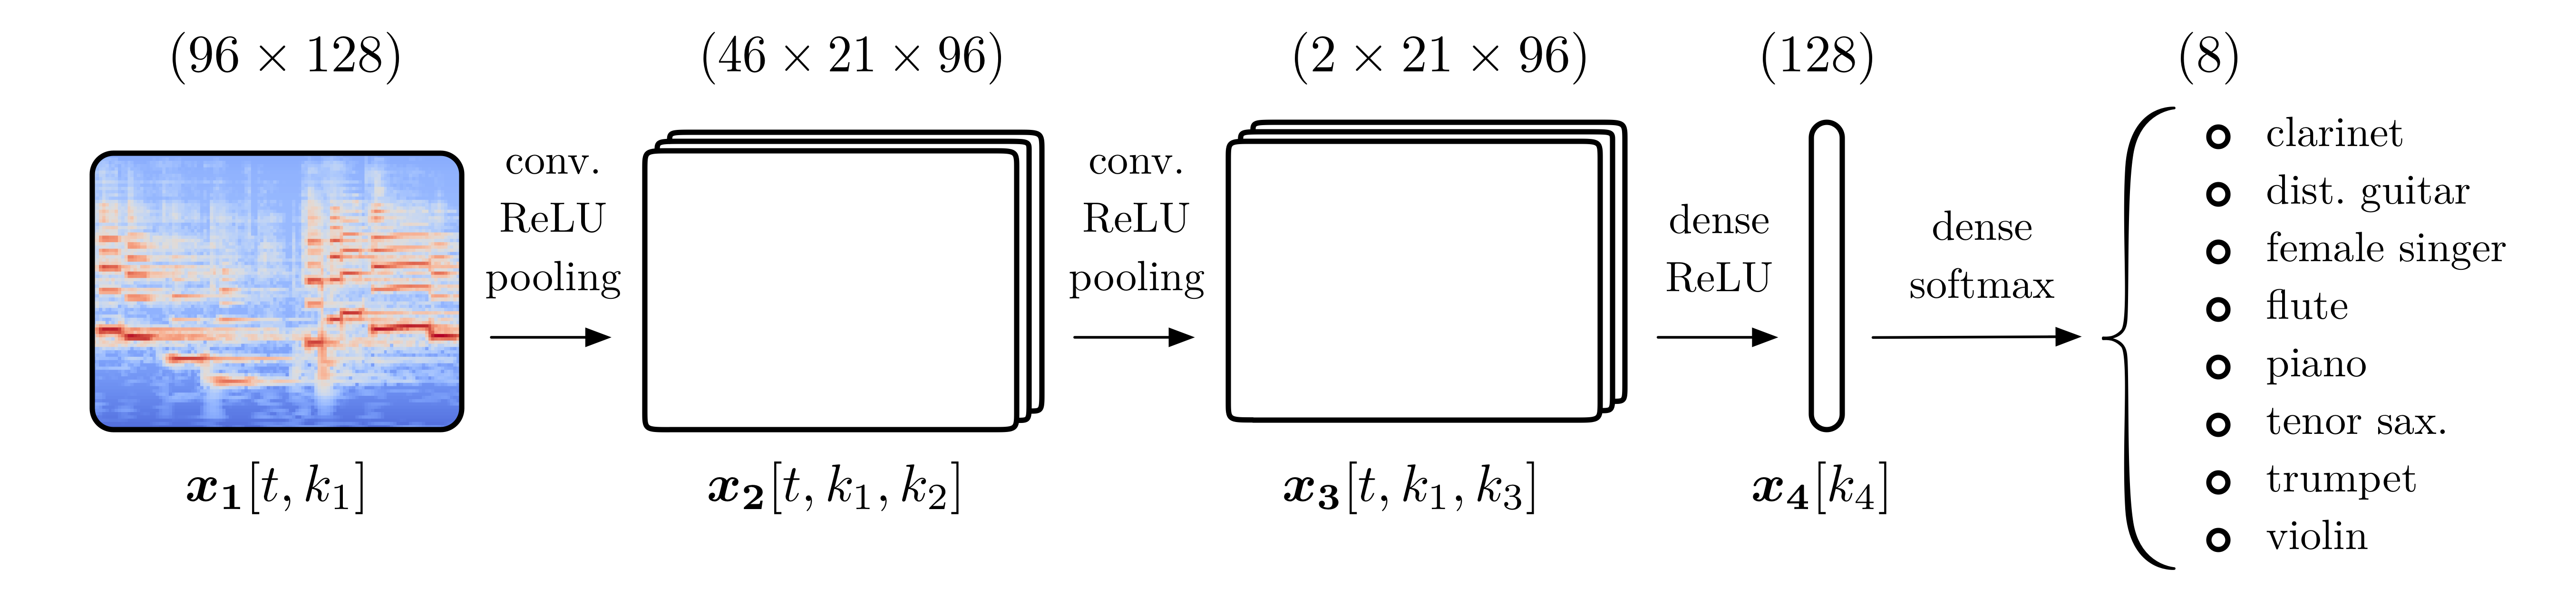
\includegraphics[width=17cm]{figs/architecture.png}}
        \end{picture}
    \end{center}
    \protect\caption{
Architecture of a convolutional network with full weight sharing. See text for details.
\label{fig:instrument-distribution}
}
\end{figure*}

The input of our system is a constant-Q wavelet scalogram, which is very comparable to a mel-frequency spectrogram.
We used the implementation from the librosa package \cite{McFee2015-librosa} with $Q=12$ filters per octave, center frequencies ranging from 55 Hz to 14 kHz (8 octaves from A1 to A9), and a hop size of 23 ms.
Furthermore, we applied nonlinear perceptual weighting of loudness in order to reduce the dynamic range between the fundamental partial and its upper harmonics.
A 3-second sound excerpt $\boldsymbol{x}[t]$ is represented by a time-frequency matrix $\boldsymbol{x_1}[t,k_1]$ of width $T=128$ samples and height $K_1=96$ frequency bands.

Each layer in a convolutional network typically consists in the composition of three operations: two-dimensional convolutions, application of a pointwise nonlinearity, and local pooling. A convolutional operator is defined as a family $\boldsymbol{W_2}[\tau,\kappa_1,k_2]$ of $K_2$ two-dimensional filters, whose impulse repsonses are all constrained to have width $\Delta t$ and height $\Delta k_1$. Element-wise biases $\boldsymbol{b_2}[k_2]$ are added to the convolutions, resulting in the three-way tensor 
\begin{IEEEeqnarray}{rCl}
\IEEEeqnarraymulticol{3}{l}{
\boldsymbol{y_2}[t,k_1,k_2]} \nonumber \\
& = & \boldsymbol{b_2}[k_2] + 
\boldsymbol{W_2}[t, k_1, k_2] \overset{t,k_1}{\ast} \boldsymbol{x_1}[t, k_1]
\nonumber \\
& = &
\boldsymbol{b_2}[k_2] + 
\sum_{\substack{
0 \leq \tau < \Delta t \\
0 \leq \kappa_1 < \Delta k_1}}
\! \! \! \! \!
\boldsymbol{W_2}[\tau, \kappa_1, k_2]
\boldsymbol{x_1}[t-\tau, k_1-\kappa_1].
\IEEEeqnarraynumspace
\label{eq:convolution}
\end{IEEEeqnarray}
 The pointwise nonlinearity we have chosen the \emph{rectified linear unit} (ReLU) because of its popularity in computer vision and its computational efficiency.
 \begin{equation}
 \boldsymbol{y_{2}^{+}}[t,k_1,k_2] = \max \left( \boldsymbol{y_2}[t,k_1,k_2], 0\right)
 \label{eq:relu}
 \end{equation}
 The pooling step consists in retaining the maximal activation among neighboring units in the time-frequency domain $(t, k_1)$ over non-overlapping rectangles of width $\Delta t$ and height $\Delta k_1$.
\begin{equation}
\boldsymbol{x_2}[t,k_1,k_2] = \! \!
\max_{
\substack{
0 \leq \tau < \Delta t \\
0 \leq \kappa_1 < \Delta k_1}
} \! \!
\left\{
\boldsymbol{y_{2}^{+}}[t - \tau, k_1 - \kappa_1, k_2]
\right\}
\label{eq:pooling}
\end{equation}
The hidden units in $\boldsymbol{x_2}$ are in turn fed to a second layer of convolutions, ReLU, and pooling.
Observe that the corresponding convolutional operator $\boldsymbol{W_3}[\tau, \kappa_1, k_2, k_3]$ performs a linear combination of time-frequency feature maps in $\boldsymbol{x_2}$ along the channel variable $k_2$.
\begin{IEEEeqnarray}{rCl}
\IEEEeqnarraymulticol{3}{l}{
\boldsymbol{y_3}[t,k_1,k_3]} \nonumber \\
& = &
\sum_{k_2}
\boldsymbol{b_3}[k_2, k_3]
+ \boldsymbol{W_3}[t, k_1, k_2, k_3]
\overset{t,k_1}{\ast}
\boldsymbol{x_2}[t,k_1,k_2].
\IEEEeqnarraynumspace
\end{IEEEeqnarray}
Tensors $\boldsymbol{y_3}^{+}$ and $\boldsymbol{x_3}$ are derived from $\boldsymbol{y_3}$ by ReLU and pooling, with formulae similar to Eqs. (\ref{eq:relu}) and (\ref{eq:pooling}). The third layer consists of the linear projection of $\boldsymbol{x_3}$, viewed as a vector of the flattened index $(t, k_1, k_3)$, over $K_4$ units:
\begin{IEEEeqnarray}{rCl}
\boldsymbol{y_4}[k_4] =
\boldsymbol{b_4}[k_4] +
\sum_{t,k_1,k_3}
\boldsymbol{W_4}[t, k_1, k_3, k_4]
\boldsymbol{x_3}[t, k_1, k_3]
\label{eq:densely-connected-layer}
\IEEEeqnarraynumspace
\end{IEEEeqnarray}
We apply a ReLU to $\boldsymbol{y_4}$, yielding $\boldsymbol{x_4}[k_4] = \boldsymbol{y_4^{+}}[k_4]$.
Finally, we project $\boldsymbol{x_4}$ onto a layer of output units $\boldsymbol{y_5}$ that should represent instrument activations: $\boldsymbol{y_5}[k_5] = \sum_{k_4} \boldsymbol{W_5}[k_4, k_5] \boldsymbol{x_4}[k_4]$.
\begin{equation}
\boldsymbol{x_5}[k_5] =
\frac{\exp \boldsymbol{y_5}[k_5]}
{  \sum_{\kappa_5} \exp \boldsymbol{y_5}[\kappa_5] }
\end{equation}
The above ensures that the coefficients of $\boldsymbol{x_5}$ are non-negative and sum to one, hence can be fit to a probability distribution.
\begin{equation}
\mathscr{L}(\boldsymbol{x_5}, \mathcal{I}) =
- \sum_{k_5 \in \mathcal{I}} \log \boldsymbol{x_5}[k_5]
+ \lambda_5 \Vert W_5 \Vert
\end{equation}
The goal is to minimize the average loss $\mathscr{L}(\boldsymbol{x_5}, \mathcal{I})$ for across all pairs $(\boldsymbol{x}, \mathcal{I})$ in the training set.

% Categorical cross-entropy
% For music instrument classification, this objective function is a histogram of the active instruments within an audio stream.
The network is trained on categorical cross-entropy over shuffled mini-batches of size 64 with uniform class distribution.
Each training example is a 3-second spectrogram whose boundaries are selected at random over non-silent regions of a song. Each spectrogram within a batch was globally normalized such that the whole batch had unit mean and unit variance.
The learning rate policy for each scalar weight in the network is \emph{Adam} \cite{Kingma2015}, a state-of-the-art online optimizer for gradient-based learning.
The architecture was built using the Keras library \cite{Chollet2015}, and trained on a graphics processing unit within a few minutes.
% Ref to LeCun on disentangling factors of variability
% Ref to Newton 2012

\section{Convolutions on the pitch spiral}
"Local neighborhoods in frequency do not share the same relationship", Humphrey \etal acknowledge in their review of deep learning techniques for MIR. Indeed, since the neighboring partials of a harmonic sound are evenly spaced in frequency, they tend to get closer to each other on a mel scale. 

Let $\boldsymbol{\phi}[k_1]$ be a window function of width $2Q$, that is two octaves. We have chosen a Tukey window ($\alpha=0.5$), which has a flat top of width $Q$ surrounded by cosine tapering lobes of width $Q/2$.
\begin{IEEEeqnarray}{rCl}
\boldsymbol{y_2}[t,k_1,k_2]
= & &
\! \! \! \! \! \! \! \! \! \! \! \! \! \! \! \! \! \! \! \!
\boldsymbol{b_2}[k_2]  \nonumber \\
& +
\! \sum_{\tau, \kappa_1, j_1} \! &
\boldsymbol{W_2}[\tau, \kappa_1, j_1, k_2] \nonumber \\
& &\times
\boldsymbol{x_1}[t - \tau, k_1 - \kappa_1] \nonumber \\
& & \times
\boldsymbol{\phi}[k_1 - \kappa_1 + Q j_1].
\IEEEeqnarraynumspace
\end{IEEEeqnarray}
Compare the above with Equation (\ref{eq:convolution}).
Limited weight sharing has been introduced by Abdel-Hamid et al. \cite{Abdel-Hamid2014}.

\section{Single-instrument classification}\label{sec:single-instrument}
\subsection{Experimental design}
In order to train the proposed algorithms, we used MedleyDB v1.1. \cite{Bittner2014}, a dataset of 122 multitracks annotated with instrument activations as well as melodic $f_0$ curves when present. We extracted the monophonic stems corresponding to a selection of eight pitched instruments (see Table \ref{table:single-label-durations}). Stems with leaking instruments in the background were discarded.

The evaluation set consists of 126 recordings of solo music collected by Joder et al. \cite{Joder2009}, to which we add 23 stems of electric guitar and female voice from MedleyDB. In doing so, guitarists and vocalists were thoroughly put either in the training set or the test set, to prevent any artist bias. We discarded recordings with extended instrumental techniques, since they are under-represented in MedleyDB.

Constant-Q spectrograms from the evaluation set were split into half-overlapping, 3-second excerpts.
% The probability distribution of labels was computed for every excerpt in a track, and then 


\begin{table}
	\begin{center}
	\begin{tabular}{|c|cc|cc|}
		\hline
		& minutes & tracks & minutes & tracks \\
		\hline
		clarinet & 10 & 7 & 13 & 18 \\
		dist. guitar & 15 & 14 & 17 & 11 \\
		female singer & 10 & 11 & 19 & 12 \\
		flute & 7 & 5 & 53 & 29 \\
		piano & 58 & 28 & 44 & 15 \\
		tenor sax. & 3 & 3 & 6 & 5 \\
		trumpet & 4 & 6 & 7 & 27 \\
		violin & 51 & 14 & 49 & 22 \\
		\hline
		total & 158 & 88 & 208 & 139 \\
		\hline
	\end{tabular}
	\end{center}
	\caption{\label{table:single-label-durations}}
\end{table}

\subsection{Results}
Results are charted in Table \ref{table:single-label-results}.

\begin{table}
	\begin{center}
	\begin{tabular}{|l|c|}
		\hline
		Representation & Error rate (\%) \\
		\hline
		MFCC \& random forest & $-$ \\
		ConvNet, full weight sharing & $-$ \\
		ConvNet, limited weight sharing & $-$ \\
		\hline
	\end{tabular}
	\end{center}
	\caption{\label{table:single-label-results}}
\end{table}

\section{Conclusions}
Understanding the influence of pitch in audio streams is paramount to the design of an efficient system for automated classification, tagging, and similarity retrieval in music. 
We have presented a data-driven, supervised method to address pitch invariance while preserving good timbral discriminability.
Future work will be devoted to integrating the proposed scheme with other advances in deep learning for music informatics, such as data augmentation \cite{McFee2015-muda}, multiscale representations \cite{Hamel2012, Anden2015}, and adversarial training \cite{Kereliuk2015}.
% For bibtex users:
\bibliography{ISMIR2015template}

\end{document}
